\section{Homotopia}
\label{homotopia}
Um assunto que aparece na definição de objetos importantes na topologia algébrica, como os grupos de homotopia e, em particular, o grupo fundamental.

%---------------------------------------------------------------------------------------------------------------------!Draft!-----------------------------------------------------------------------------------------------------------------
\subsection{Homotopia}
\label{homotopia-def}
%\begin{titlemize}{Lista de dependências}
	%\item \hyperref[dependecia1]{Dependência 1};\\ %'dependencia1' é o label onde o conceito Dependência 1 aparece (--à arrumar um padrão para referencias e labels--) 
	%\item \hyperref[]{};\\
% quantas dependências forem necessárias.
%\end{titlemize}
\begin{defi}[Homotopia]
	Sejam $X$ e $Y$ espaços topológicos. Uma homotopia entre funções contínuas $f_0, f_1: X\rightarrow Y$ é uma função $$H:X\times I\rightarrow Y$$ também contínua tal que $H(x,0)=f_0(x)$ e $H(x,1)=f_1(x)$. Se existe homotopia entre os mapas $f_0$ e $f_1$, dizemos que $f_0$ é homotópico a $f_1$, e escrevemos $f_0\sim f_1$. Quando quisermos explicitar que $f_0$ é homotópico a $f_1$ através da homotopia $H$, escrevemos $f_0 \underset{H}{\sim} f_1$ e também $H:f_0\Rightarrow f_1$.
\end{defi}

\begin{titlemize}{Lista de consequências}
	\item \hyperref[homotopia-relaçao-de-equivalencia-prop]{Homotopia como relação de equivalência};\\ %'consequencia1' é o label onde o conceito Consequência 1 aparece
	\item \hyperref[teorema-bola-cabeluda-prop]{Teorema da bola cabeluda}
\end{titlemize}

%[Bianca]: é mais fácil criar a lista de dependências do que a de consequências.
% onde conteudos.tex é o nome do arquivo tex que voce quer incluir nessa secção.
\input{conteudo/homotopia-relativa-def}
\input{conteudo/homotopia-relaçao-de-equivalencia-prop}
%---------------------------------------------------------------------------------------------------------------------!Draft!-----------------------------------------------------------------------------------------------------------------
\subsection{Equivalência de Homotopia}
\label{equiv-homotopia}
\begin{titlemize}{Lista de dependências}
	\item \hyperref[homotopia-def]{Homotopia};\\
\end{titlemize}

\begin{defi}[Equivalência de Homotopia]
	Sejam $X$ e $Y$ espaços topológicos. Uma função contínua $f:X\to Y$ é dita uma \textbf{equivalência de homotopia} se existe outra função contínua $g:Y\to X$ tal que $f\circ g \sim \text{id}_Y$ e $g\circ f \sim \text{id}_X$. Nesse caso, dizemos que $X$ e $Y$ são \textbf{homotopicamente equivalentes}, e $g$ é \textbf{inversa a menos de homotopia} de $f$.
\end{defi}

É claro que todo homeomorfismo é uma equivalência de homotopia.

\begin{titlemize}{Lista de consequências}
    \item \hyperref[espaco-contratil-def]{Espaço contrátil}
	\item \hyperref[equiv-homotopia-induz-iso]{Equivalência de homotopia e grupo fundamental}
\end{titlemize}

%[Bianca]: é mais fácil criar a lista de dependências do que a de consequências.

\subsection{Espaço contrátil}
\label{espaco-contratil-def}
\begin{titlemize}{Lista de dependências}
	\item \hyperref[homotopia-def]{Homotopia};\\
        \item \hyperref[equiv-homotopia]{Equivalência de Homotopia}.
\end{titlemize}

\begin{defi}
	Seja $X$ um espaço topológico. Diremos que o espaço $X$ é \textbf{contrátil} se $X$ é homotopicamente equivalente a um ponto.
\end{defi}

Ou seja, um espaço topológico $X$ é contrátil se existem $f:\{*\} \to X$ e $g: X\to \{*\}$ tais que $g\circ f \sim \text{id}_X$ e $f\circ g \sim \text{id}_{\{*\}}$. Mas como $f\circ g = \text{id}_{\{*\}}$, e substituindo $f:\{*\} \to X$ pela inclusão $\{f(*)\} \hookrightarrow X$, concluímos que $X$ é contrátil se, e somente se, existem $x_0\in X$ e $H: X\times I\to X$ tais que $H(x,0)=x$ e $H(x,1) = x_0$ para todo $x \in X$.

\begin{ex}
    \begin{itemize}
        \item $D^n$ é contrátil, para todo $n\geq 0$, %. Sejam $f: D^n\to\{0\}$ e $g:\{0\}\hookrightarrow D^n$. Então $f\circ g$ é a identidade em $\{0\}$ e $g\circ f$ é homotópico à identidade em $D^n$,
        via
        \begin{align*}
            H: D^n \times I &\to D^n\\
            (x,t) &\mapsto (1-t)x.
        \end{align*}
        \item Mais geralmente, se $S \subset \mathbb{R}^n$ é um subconjunto estrelado, então é contrátil. Seja $s_0\in S$ tal que $ts + (1-t)s_0 \in S$ para todos $t\in I$ e $s\in S$. Como $S-s_0 = \{s-s_0~|~s\in S\} \cong S$, podemos supor que $s_0 = 0$. %Além disso, note que, como $\mathbb{R}^n$ e $\text{int}(D^n)$ são homeomorfos, podemos supor que $S \subset D^n$. %<-- acho que não precisa
        Assim, definimos
        \begin{align*}
            H: S \times I &\to S\\
            (x,t) &\mapsto (1-t)x.
        \end{align*}
        %e concluímos como no caso anterior.
        \item Dado um espaço topológico $X$, o cone $C(X)$ é contrátil. Para ver isso, seja $v$ o vértice do cone e defina%, $f: C(X)\to\{v\}$ e $g: \{v\}\to C(X)$. Então $f\circ g$ é a identidade em $\{v\}$ e $g\circ f$ é homotópico à identidade em $C(X)$, pois
        \begin{align*}
            \text{id}_X\times m: X\times I \times I &\to X\times I\\
            (x,s,t) &\mapsto (x,st).
        \end{align*}
        Então $\text{id}_X\times m$ induz $H_0: C(X)\times I\to X\times I$ dada por $([x,s],t) \mapsto (x,st)$. Assim, definimos $H = \pi \circ H_0$, onde $\pi: X\times I \to C(X)$ é a aplicação quociente.
    \end{itemize}
\end{ex}
\subsection{lema-teo-fundamental-da-algebra} 
\label{lema-teo-fundamental-da-algebra}
\begin{titlemize}{Lista de dependências}
	\item \hyperref[homotopia]{homotopia};\\  
	\item \hyperref[grupo-fundamental]{grupo-fundamental};\\
    \item \hyperref[retração]{retração};

\end{titlemize}
O próximo lema será uma das bases para a demonstração do Teorema Fundamental da Álgebra.
\begin{thm}[Lema] 
	Seja $\mathbb{C}$ o conjunto dos números complexos e $r\mathbb{S}^1 \subseteq \mathbb{R}^2 \cong \mathbb{C}$ a esfera centrada em 0 e de raio $r$. Sejam $f_r^n: r\mathbb{S}^1 \rightarrow \mathbb{C}\backslash \{0\}$ as restrições das funções que levam $z$ em $z^n$. Se nenhuma das funções é homotópica a uma função constante, então vale o Teorema Fundamental da Álgebra, ou seja, todo polinômio com grau maior ou igual a 1 tem raiz complexa.
	
\end{thm}

\begin{dem}
    Seja $g(z) = a_nz^n + a_{n - 1}z^{n - 1} +...+ a_0$
um polinômio com raízes complexas e com $a_n \neq 0$. Sem perda de generalidade, podemos supor $a_n = 1$ (basta tomar $h(z) = \frac{g(z)}{a_n}$).\\ Seja $r > max\{1, \sum_{i = 1}^n|a_i|\}$ e defino $F:r\mathbb{S}^1\times I \rightarrow \mathbb{C}$ como

$$F(z, t) = z^n + \sum_{i = 1}^{n-1}(1 - t)a_iz^i$$

Nota-se facilmente que $F$ é homotopia de $f_r^n$ e $g|_{r\mathbb{S}^1}$. Ainda, o contradomínio da $F$ é $\mathbb{C}\backslash \{0\}$, pois se não, haveria $z_0$ com $|z_0| = r$ e $t_0 \in I$, tal que $F(z_0, t_0) = 0$, i.e. $z_0^n = -\sum_{i = 1}^{n - 1}(1 - t_0)a_iz^i$ e, então, 

$$|z_o^n| = r^n \leq \sum_{i = 1}^{n - 1}|(1 - t_0)a_iz_0^i| \leq \sum_{i = 1}^{n - 1}|a_iz_0^i| \leq r^{n-1}\sum_{i = 1}^{n - 1}|a_i|$$

que implicaria $r \leq \sum_{i = 1}^{n - 1}|a_i|$, contradizendo a escolha de $r$.

Agora, por contrapositiva, assumimos que $g$ não tem raízes complexas, i.e. $g:\mathbb{C} \rightarrow \mathbb{C}\backslash\{0\}$. Seja $G: r\mathbb{S}^1\times I \rightarrow \mathbb{C}\backslash\{0\}$ definida por $g((1 - t)z)$. Temos que $g \sim_G c$, onde $c(z) = g(0) = a_0$ para todo $z \in r\mathbb{S}^1$. Assim, temos que $f_r^n \sim_G c$ por transitividade, garantindo a contrapositiva.  

\end{dem}
A restrição no contradomínio da $f_r^n$ é importante, pois se o contradomínio for contrátil, então qualquer função é homotópica a uma constante. De fato, se $f:X \rightarrow Y$ e $Y$ é contrátil, então $1_Y \sim_H k$, onde $k$ é uma função constante e $H$ é homotopia. Então, $f\circ1_Y \sim_H f\circ k$ e, portanto, $f \sim_H f(k_0)$, onde $k_0 = k(z)$. \\

Note também que a homotopia de $g|_{r\mathbb{S}^1}$ e $f_r^n$ deforma continuamente a imagem do polinômio que, restrito a $r\mathbb{S}^1$, torna-se uma curva fechada no plano dos complexos, no círculo de raio $r$ em $\mathbb{C}$. Veja a imagem abaixo.

\begin{figure}[h]
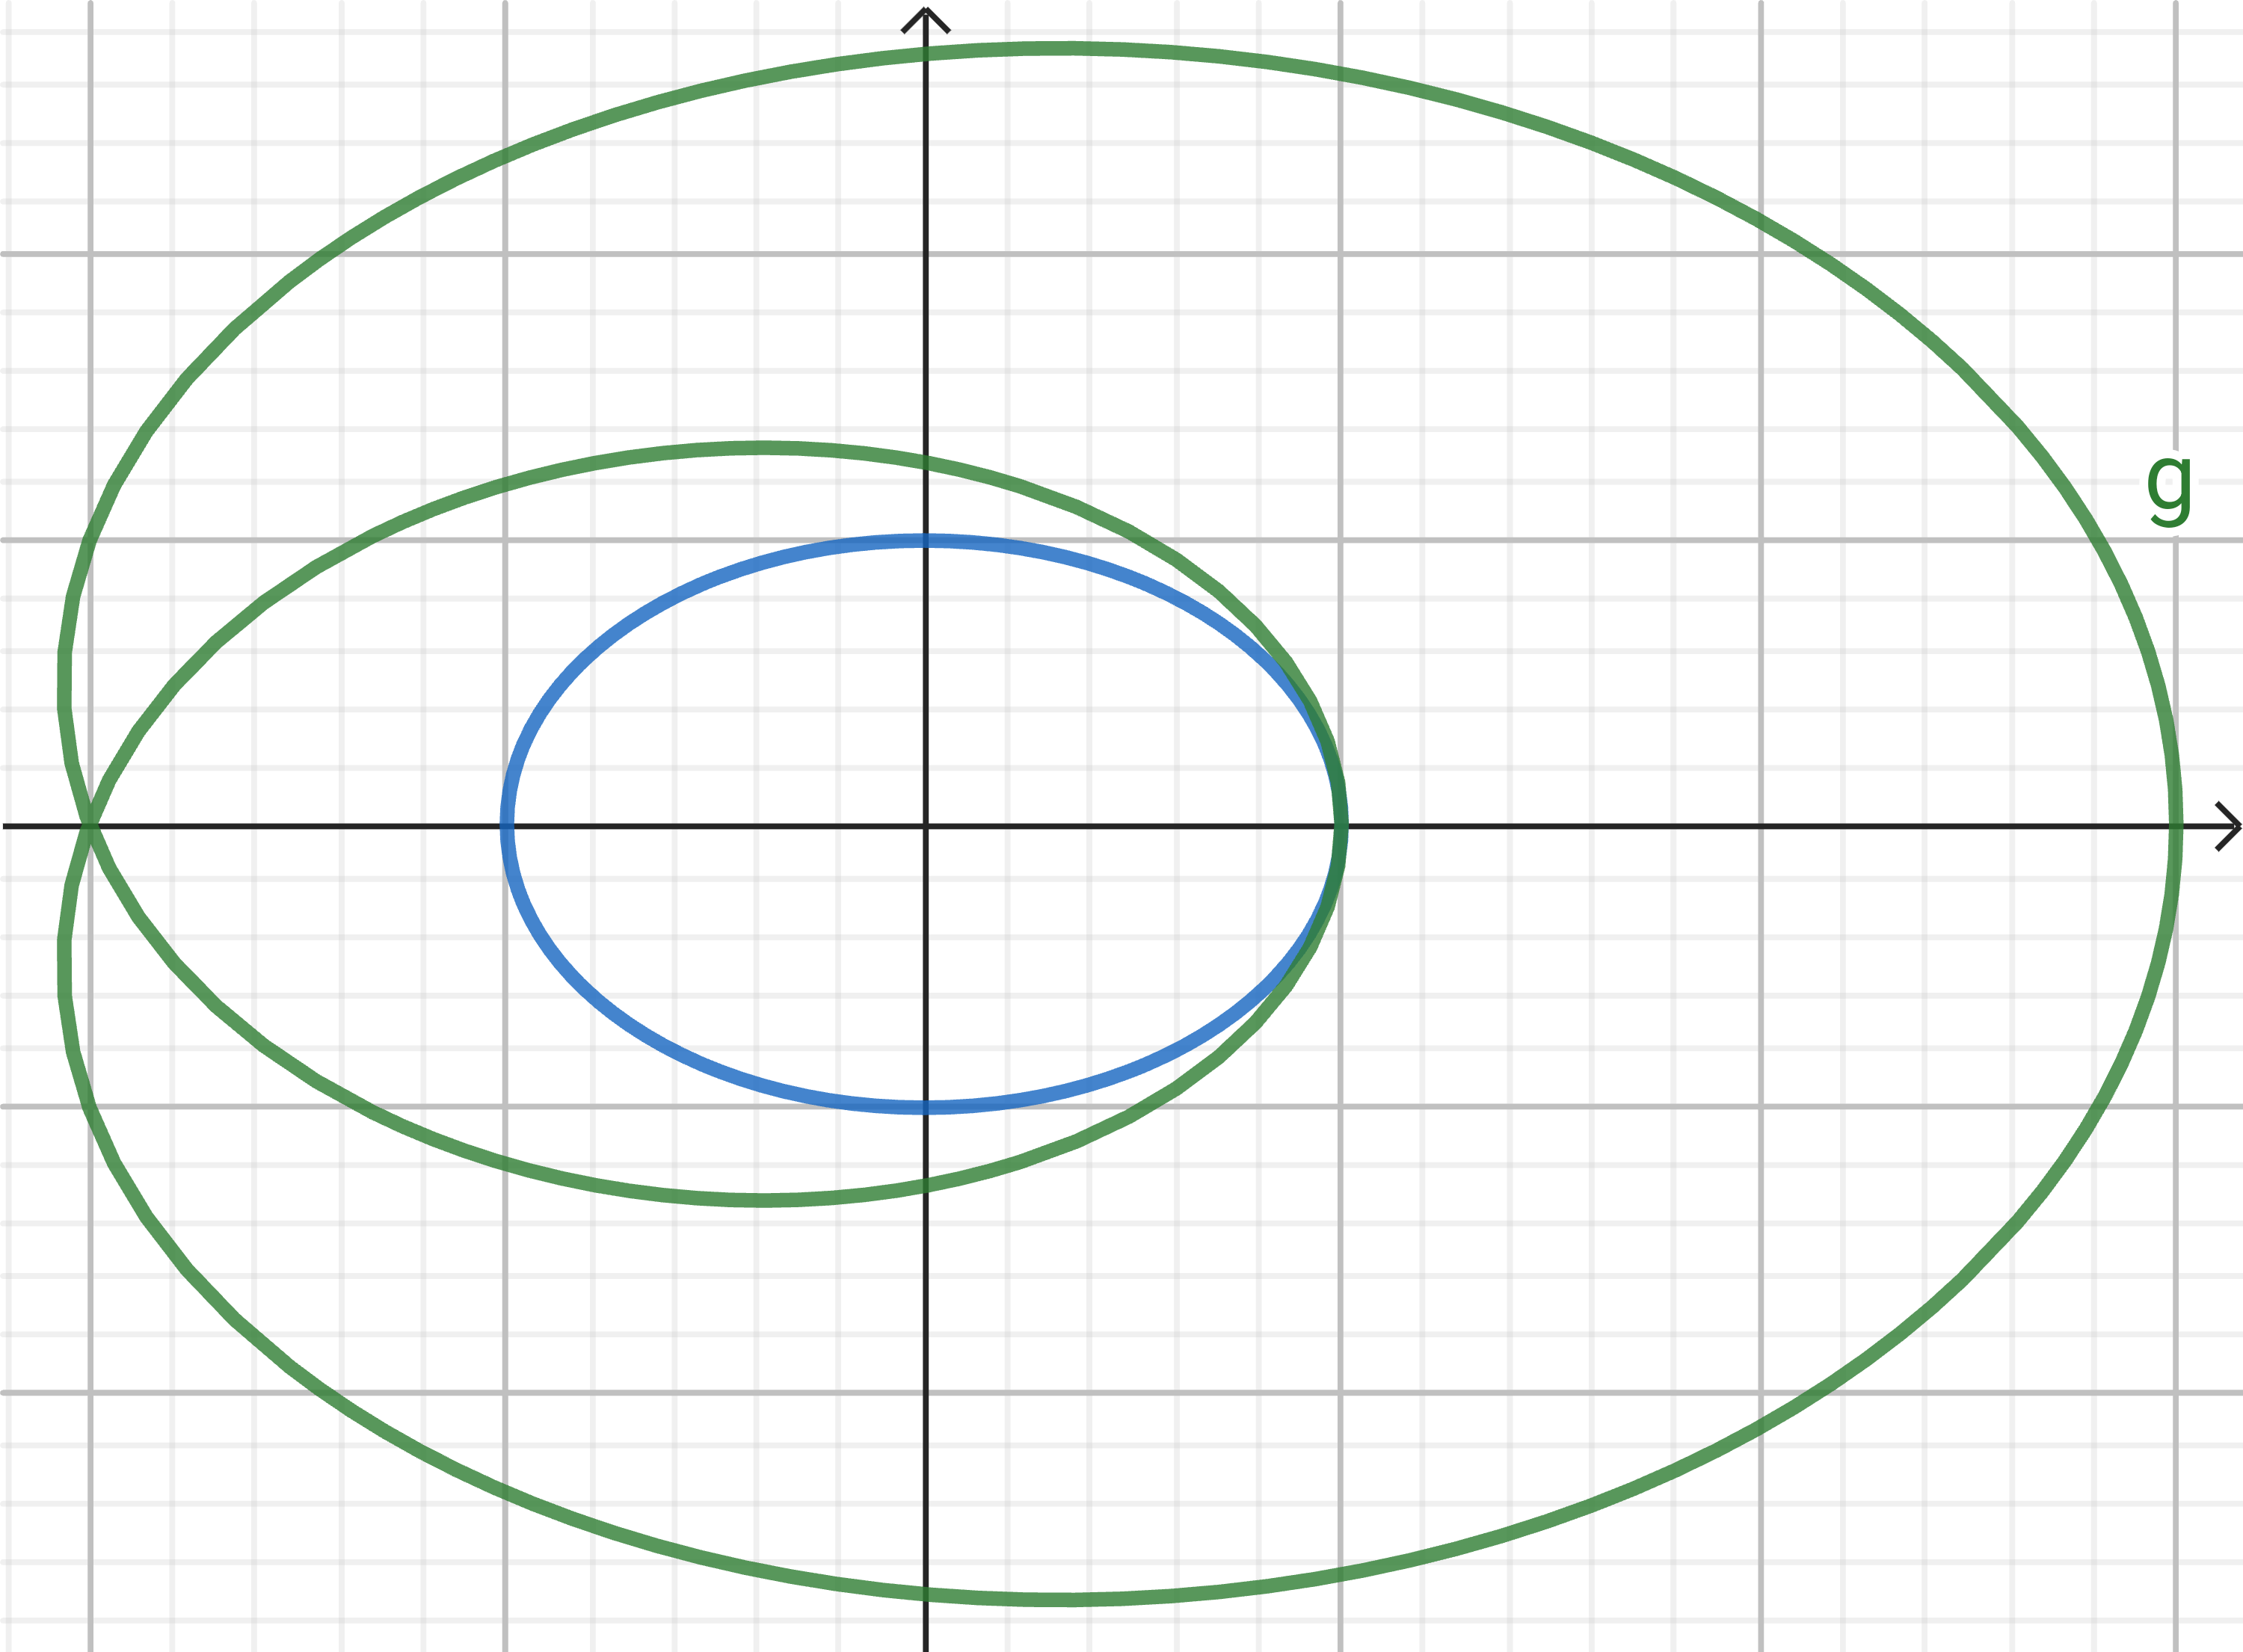
\includegraphics[width = 5cm]{conteudo/homotopia.png}
\end{figure}

\begin{titlemize}{Lista de consequências}
	\item \hyperref[teo-fundamental-da-algebra]{teo-fundamental-da-algebra};\\ 
	
\end{titlemize}

\subsection{teo-fundamental-da-algebra} %afirmação aqui significa teorema/proposição/colorário/lema
\label{teo-fundamental-da-algebra}
\begin{titlemize}{Lista de dependências}
	\item \hyperref[lema-teo-fundamental-da-algebra]{lema-teo-fundamental-da-algebra};\\ %'dependencia1' é o label onde o conceito Dependência 1 aparece (--à arrumar um padrão para referencias e labels--) 
	\item \hyperref[extensão-de-função-na-esfera]{extensão-de-função-na-esfera};\\
  \item \hyperref[grupo-fundamental-de-S1-prop]{grupo-fundamental-de-S1-prop}
\end{titlemize}
\begin{thm}[Teorema Fundamental da Álgebra]

	Todo polinômio não constante com coeficientes complexos possui raíz em $\mathbb{C}$. \\
 
 Em outras palavras, esse teorema garante que o corpo dos complexos é um fecho algébrico dos corpos de característica 0.
 
\end{thm}

\begin{dem}

Pelo lema referenciado na lista de dependências, basta mostrar que as funções $f_r^n: r\mathbb{S}^1 \rightarrow \mathbb{C}\backslash\{0\}$, definidas por $f_r^n(z) = z^n$, não são homotópicas a uma constante.
De fato, caso $f_r^n$ fosse homotópica a uma constante, então $h: \mathbb{S}^1 \rightarrow r\mathbb{S}^1 \rightarrow \mathbb{C}\backslash\{0\} \rightarrow \mathbb{S}^1$ dada por $h(z) = \frac{f_r^n(rz)}{|f_r^n(rz)|}$ também seria homotópica a uma constante, já que se $H:r\mathbb{S}^1 \times I \rightarrow \mathbb{C}\backslash\{0\}$ é a homotopia entre $f_r^n$ e uma constante $c_0$, então $\frac{1}{r^n}H(rz, t)$ é homotopia entre $h$ e $\frac{c_0}{r^n}$.\\
No entanto, por uma das equivalências de \hyperref[extensão-da-função-na-esfera]{extensão-da-função-na-esfera}, se $h$ é homotópica a uma constante, então $h_*$ é trivial, implicando que $h_*([e^{2\pi i}])$ é elemento neutro em $\mathcal{S}^1$, ou seja $[e^{2\pi in}] = [1]$ e, portanto, com a linguagem do levantamento de homotopia na seção do grupo fundamental de $\mathbb{S}^1$, temos que $deg([e^{2\pi in]}) = deg([1]) = 0$, contrariando o fato de que, na verdade, $deg([e^{2\pi in}]) = n$. Portanto, $f_r^n$ não pode ser homotópico a uma constante e, dessa forma, vale o Teorema Fundamental da Álgebra.

    
\end{dem}

Note que a interpretação geométrica de $h$ é de alongar os pontos em $\mathbb{S}^1$, aumentando o seu raio, e depois rotacioná-los e contraí-los de volta a $\mathbb{S}^1$. A homotopia de $h$ à constante deforma continuamente a circunferência de raio $1$ no ponto $c_0$, trazendo-o mais próximo da origem.

%---------------------------------------------------------------------------------------------------------------------!Draft!-----------------------------------------------------------------------------------------------------------------
\subsection{Identidade e antípoda são homotópicas se há campo não nulo} %afirmação aqui significa teorema/proposição/colorário/lema
\label{identidade-e-antipoda-homotopicas-prop}
\begin{titlemize}{Lista de dependências}
	\item \hyperref[homotopia-def]{Homotopia};\\ %'dependencia1' é o label onde o conceito Dependência 1 aparece (--à arrumar um padrão para referencias e labels--) 
	%\item \hyperref[]{};\\
% quantas dependências forem necessárias.
\end{titlemize}




\begin{lemma}[Funções identidade e antípoda na esfera]% ou af(afirmação)/prop(proposição)/corol(corolário)/lemma(lema)/outros ambientes devem ser definidos no preambulo de Alg.Top-Wiki.tex 
	Se existe uma função contínua $v:S^n\rightarrow \mathbb{R}^{n+1}$ que leva todo $x\in S^n$ em $v(x)$ com $\langle x, v(x) \rangle =0$, isto é, um campo vetorial contínuo não nulo tangente à esfera, então as funções identidade $Id_{S^n}:S^n\rightarrow S^n$ e antípoda $A_{S^n}:S^n\rightarrow S^n$ dada por $A_{S^n}(x)=-x$ para todo $x\in S^n$ são homotópicas.
\end{lemma}
\begin{dem}
    Seja $v:S^n\rightarrow \mathbb{R}^{n+1}$ o campo vetorial contínuo tangente à esfera que é não nulo em todos os pontos e considere a função contínua $H:S^n\times I\rightarrow S^n$ definida por $$H(x,t)=cos(\pi t)x+sen(\pi t)\frac{v(x)}{||v(x)||}.$$
    De fato, $H$ está bem definida pois, utilizando o fato de que $\langle x, v(x) \rangle =0$, temos 

    $$|cos(\pi t)x+sen(\pi t)\frac{v(x)}{||v(x)||}|^2=$$$$=\langle cos(\pi t)x+sen(\pi t)\frac{v(x)}{||v(x)||} , cos(\pi t)x+sen(\pi t)\frac{v(x)}{||v(x)||}\rangle=$$$$=cos^2(\pi t)\langle x,x \rangle +sen^2(\pi t)\langle \frac{v(x)}{||v(x)||},\frac{v(x)}{||v(x)||}\rangle=$$$$=cos^2(\pi t)+sen^2(\pi t)=1.$$
    
    Isto é, $H(x,t)$ pertence à esfera para todo $(x,t)\in X\times I$. Além disso, $H$ é homotopia entre a identidade e a antípoda pois $$H(x,0)=cos(0)x+sen(0)\frac{v(x)}{||v(x)||}=x=Id(x)\text{ para todo } x\in S^n$$ $$\text{e } H(x,1)=cos(\pi)x+sen(\pi)\frac{v(x)}{||v(x)||}=-x=A(x)\text{ para todo }x\in S^n.$$
\end{dem}


\begin{titlemize}{Lista de consequências}
	\item \hyperref[teorema-bola-cabeluda-prop]{Teorema da Bola Cabeluda};\\ %'consequencia1' é o label onde o conceito Consequência 1 aparece
	%\item \hyperref[]{}
\end{titlemize}

%[Bianca]: Um arquivo tex pode ter mais de uma afirmação (ou definição, ou exemplo), mas nesse caso cada afirmação deve ter seu próprio label. Dar preferência para agrupar afirmações que dependam entre sí de maneira próxima (um teorema e seu corolário, por exemplo)

%---------------------------------------------------------------------------------------------------------------------!Draft!-----------------------------------------------------------------------------------------------------------------
\subsection{Teorema da Bola Cabeluda} %afirmação aqui significa teorema/proposição/colorário/lema
\label{teorema-bola-cabeluda-prop}
\begin{titlemize}{Lista de dependências}
	\item \hyperref[homotopia-def]{Homotopia};\\ %'dependencia1' é o label onde o conceito Dependência 1 aparece (--à arrumar um padrão para referencias e labels--) 
	\item \hyperref[identidade-e-antipoda-homotopicas-prop]{Homotopia entre identidade e antípoda};\\
% quantas dependências forem necessárias.
\end{titlemize}


\begin{thm}[Teorema da Bola Cabeluda]% ou af(afirmação)/prop(proposição)/corol(corolário)/lemma(lema)/outros ambientes devem ser definidos no preambulo de Alg.Top-Wiki.tex 
	A esfera $S^n$ possui um campo vetorial contínuo não nulo em todo ponto isto é, existe uma função contínua $v:S^n\rightarrow \mathbb{R}^{n+1}$ que leva todo $x\in S^n$ a $v(x)$ com $\langle x, v(x) \rangle =0$ e $v(x)\ne 0$, se e somente se $n$ é ímpar.\\
\end{thm}
\begin{dem}
    Se $n$ é ímpar, $n=2k-1$ para algum natural $k$ e basta tomar o campo $$v(x_1,~...,~x_{2k})=(-x_2,~x_1,~-x_4,~x_3,~...,~-x_{2k},~x_{2k-1})\text{ para todo }(x_1,~...,~x_{2k})\in S^n.$$
    De fato, a função é contínua, temos $$\langle(-x_2,~x_1,~...,~-x_{2k},~x_{2k-1}), (x_1,~x_2,~...,~x_{2k-1},~x_{2k}) \rangle =$$$$=-x_1x_2+x_1x_2-...-x_{2k-1}x_{2k}+x_{2k-1}x_{2k}=0$$ e vale $v(x)\ne 0$ para todo $x=(x_1,...,x_{2k})\in S^n$ pois $v(x)=(x_1,~x_2,~...,~x_{2k-1},~x_{2k})=0$ somente se $x_i=0$ para todo $i\in {1,~...,~2k}$, isto é, $v(x)=0$ apenas em ponto fora da esfera.\\

    Reciprocamente, se a esfera $S^n$ possui campo vetorial contínuo não nulo em cada ponto conforme condição do enunciado, segundo o lema \ref{identidade-e-antipoda-homotopicas-prop}, existe uma homotopia entre os mapas identidade e antípoda na esfera, o que não pode ocorrer de $n$ for par.

    
\end{dem}

Vale ressaltar que é possível demostrar que de fato não há homotopia entre a identidade e a antípoda em esferas de grau par através da noção de grau de uma função, existente em homologia. Esse tópico não será abordado neste material.

\begin{titlemize}{Lista de consequências}
	\item \hyperref[consequencia1]{Consequência 1};\\ %'consequencia1' é o label onde o conceito Consequência 1 aparece
	%\item \hyperref[]{}
\end{titlemize}

%[Bianca]: Um arquivo tex pode ter mais de uma afirmação (ou definição, ou exemplo), mas nesse caso cada afirmação deve ter seu próprio label. Dar preferência para agrupar afirmações que dependam entre sí de maneira próxima (um teorema e seu corolário, por exemplo)
%%% Local Variables:
%%% mode: LaTeX
%%% TeX-master: "../Alg.Top-Wiki"
%%% End:
